\section{Mechanische Konstruktion und Fertigung}
Die mechanische Basis des Systems bildet eine Multiplexplatte, die als tragende Struktur dient.  
Auf dieser Grundplatte werden die \gls{led}-Streifen montiert und die Frontabdeckung verschraubt.  
Der Mikrocontroller wird auf der Rückseite der Platte befestigt.  
Für die Darstellung der Wortmatrix werden Bauteile mit der \gls{cad}-Software Inventor Professional 2026 von Autodesk konstruiert (vgl. Abb.~\ref{fig:Frontplatte}).  
Es existieren Mittelteile, Eckstteile und Seitenteile (vgl. Abb.~\ref{fig:Frontplatte}).  
Alle Bauteile des selben Typs folgen demselben konstruktiven Prinzip, unterscheiden sich jedoch in der jeweiligen Buchstabenbelegung oder Symbolik.  
In Abbildung~\ref{fig:Frontplatte} ist die Gesamte Frontplatte in der \gls{cad}-Software dargestellt.

\begin{figure}[H]
	\centering
	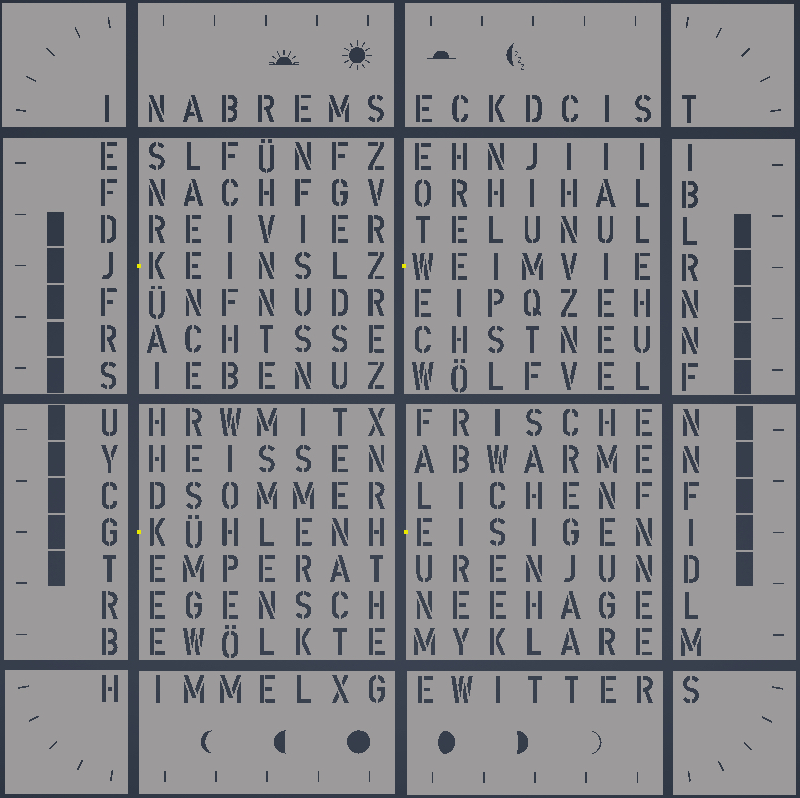
\includegraphics[width=0.6\linewidth]{inhalt/bilder/CADUhrKomplett.png}
	\caption{Gesamte Frontplatte in der CAD-Software, bestehend aus vier Eckteilen, acht Seitenteilen und vier Mittelteilen.}
	\label{fig:Frontplatte}
\end{figure}

Auf der Innenseite besitzt jeder Buchstabe eine eigene, abgeschlossene Box, damit keine anderen Buchstaben als der angesteuerte beleuchtet werden.
Dies Boxen sind in Abbildung~\ref{fig:3DDruckbeispiel} zu sehen.

Die konstruierten Bautel werden mit einem \gls{3ddruck} aus schwarzem \gls{pla} hergestellt.
Ein Beispiel dafür ist in Abb.~\ref{fig:3DDruckbeispiel} dargestellt.
\begin{figure}[H]
	\centering
	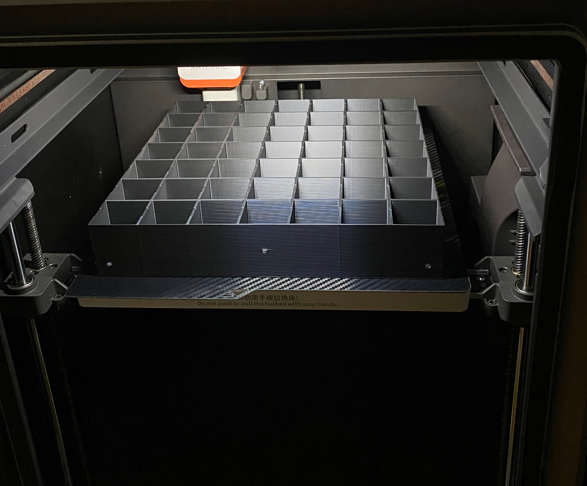
\includegraphics[width=0.5\linewidth]{inhalt/bilder/Bauteil11_gedruckt.png}
	\caption{Fertiggestellter Druck des Frontplattenbauteil Nr. 11 auf dem 3D-Drucker Kobra S1 der Marke Anycubic~\cite{KobraS1}.}
	\label{fig:3DDruckbeispiel}
\end{figure}
Die gedruckten Bauteile bilden die Frontplatte sowie die Einhausung der \gls{led}s.  
Die Konstruktion basiert auf einer modularen Struktur aus insgesamt 16 Einzelteilen (vgl. Abb.~\ref{fig:Frontplatte}), welche miteinander verschraubt werden.  
Dadurch entsteht eine zusammenhängende Frontabdeckung mit den Abmessungen H x B x T\todo{Maße angeben}.    

Die Hauptanzeige, die aus 16 mal 16 Buchstaben besteht, dient der Darstellung der Uhrzeit, der Außentemperatur und des Wetters.  
Zusätzlich werden Symbole für die Zusatzfunktionen integriert, welche links, rechts, ober- und unterhalb der Buchstabenmatrix angeordnet sind (vgl. Abb.~\ref{fig:Frontplatte}).  
Diese umfassen die Anzeige von Raumfeuchtigkeit, Innenraumtemperatur, Mondphase und Tageszeit (vgl. Abb.~\ref{fig:Frontplatte}).  
Die Sekundenanzeig ist am Ausenrand der Frontplatte mit 60 Schlitzen realisiert (vgl. Abb.~\ref{fig:Frontplatte}).

Zur Verbesserung der Lichtverteilung werden für jeden Buchstaben sowie jedes Symbol separate Diffusorplättchen konstruiert (vgl. Abb.~\ref{fig:Diffusor}).  
Diese werden ebenfalls im 3D-Druckverfahren aus weißem \gls{pla} hergestellt und dann eingeklebt.  
Die Plättchen besitzen eine Dicke von 0.4 mm, was einer Layerhöhe von 2 entspricht. 
Das bedeutet, der Drucker druckt nur 2 Schichten \gls{pla} übereinander.  
Die optimale Dicke wurde empirisch ermittelt, um eine gleichmäßige Lichtstreuung ohne signifikante Helligkeitsverluste zu erreichen.  

\begin{figure}[H]
    \centering
    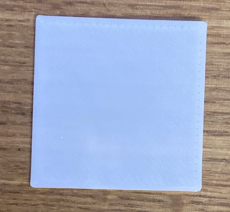
\includegraphics[width=0.5\linewidth]{inhalt/bilder/Diffusorplaettchen.png}
    \caption{3D gedrucktes Diffusorplättchen mit einer dicke von 0,4 mm.}
    \label{fig:Diffusor}
\end{figure}  

Außerdem werden Halterungen und Kleinteile für verschieden Anwendungszwecke Konstruiert und gedruckt.
Eine Halterung wird für den \gls{dht22} benötigt um diesen an der Rückseite der WordClock anbringen zu können, damit die Innenraumtemperaturen und die Luftfeuchtigkeit am Installationsort der WordClock gemessen wird (vgl. Abb.~\ref{fig:DHT22Halter}).
Zusätzlich werden Bauteile als Abstandshalter zur Wand und gleichzeitig als Aufhängungspunkte konstruiert (vgl. Abb.~\ref{fig:Abstandshalter}).   
Weiterhin wird eine Halterung für den Mikrocontroller entwickelt, welche an der Rückseite der Multiplexplatte montiert ist.  
Dadurch bleibt die \gls{usb-c}-Schnittstelle des Mikrocontroller auch im montierten Zustand erreichbar (vgl. Abb.~\ref{fig:MontageplatteESP}).
Zuletzt wird noch eine Halterung für die Hohlsteckerbuchse, über welche die WordClock mit 5V Spannung versorgt wird, konstruiert.
Diese wird ebenfalls an der Rückseite montiert, dass der Hohlstecker des +5V Netzteils ein und ausgesteckt werden kann, ohne die WordClock von der Wand zu nehmen (vgl. Abb.~\ref{fig:HohlsteckerHalter}).

\begin{figure}[H]
    \centering
    \begin{subfigure}[t]{0.4\textwidth}
        \centering
        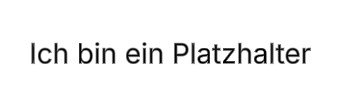
\includegraphics[width=\linewidth]{inhalt/bilder/Platzhalter.jpg}
        \caption{3D gedruckte Halterung für den \gls{dht22} um die Installationsort bezogenen Sensordaten zu erhalten.}
        \label{fig:DHT22Halter}
    \end{subfigure}
    \hfill
    \begin{subfigure}[t]{0.4\textwidth}
        \centering
        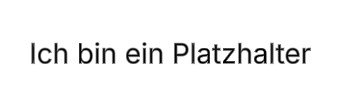
\includegraphics[width=\linewidth]{inhalt/bilder/Platzhalter.jpg}
        \caption{3D gedruckte Abstandshalter und Befestigungspunkte der WordClock, welche oben links und rechts befestigt werden um die WordClock an die Wand zu hängen. Zusätzlich 2 Abstandshalter welche unten links und rechts angebracht werden.}
        \label{fig:Abstandshalter}
    \end{subfigure}
    \vspace{0.8em}
    \begin{subfigure}[t]{0.4\textwidth}
        \centering
        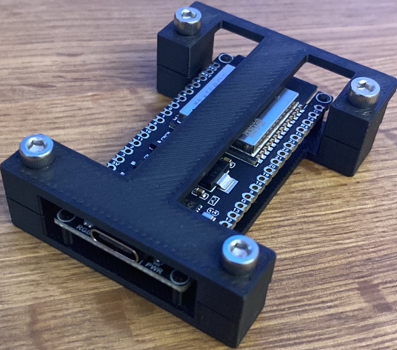
\includegraphics[width=\linewidth]{inhalt/bilder/ESPHalterEckView.png}
        \caption{3D gedruckte Montageplatte für den \gls{esp32c6}, welche an der Rückseite montiert wird.}
        \label{fig:MontageplatteESP}
    \end{subfigure}
    \hfill
    \begin{subfigure}[t]{0.4\textwidth}
        \centering
        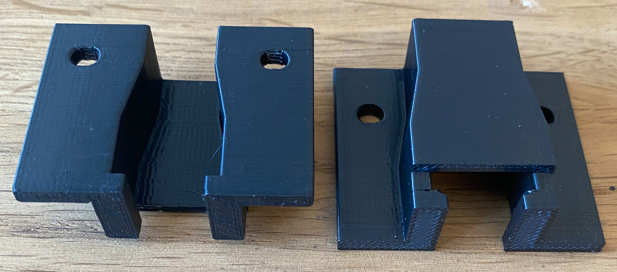
\includegraphics[width=\linewidth]{inhalt/bilder/VersorgungsanschlussHalter.png}
        \caption{Halterung für die Hohlsteckerbuchse an der WordClock zur Spannungsversorung mit +5~V.}
        \label{fig:HohlsteckerHalter}
    \end{subfigure}
    \caption{Zusätzliche Kleinteile und Halterungen der WordClock.}
    \label{fig:Kleinteile}
\end{figure}\todo{EinBildFehlt}